\chapter*{Совместные события на установках ДЕКОР и НЕВОД-ШАЛ}
\addcontentsline{toc}{chapter}{Совместные события на установках ДЕКОР и НЕВОД-ШАЛ}
\label{ch:intro}
Были отобраны события, зарегистрированные на установках ДЕКОР и НЕВОД-ШАЛ за период с 19.12.2018 по 02.02.2019, в пределах временного интервала \(|\Delta t| = |t_{\text{Д}} - t_{\text{НШ}}|  < 1000\) нс, где 

\begin{itemize}
    \item \(t_{\text{Д}}\) время регистрации события ДЕКОР,
    \item \(t_{\text{НШ}}\) время регистрации события НЕВОД-ШАЛ.
\end{itemize}
Было найдено 5214 события. Создана база данных MongoDB найденных совместных событий установок. Среднее значение временного интервала составило \( \mu_t = 336.8 \) нс, а среднее отклонение \( \sigma = 52.8 \) нс. На рисунке 5 представлено распределение совместных событий по \(\Delta t\).
\begin{figure}[ht]
    \centering
    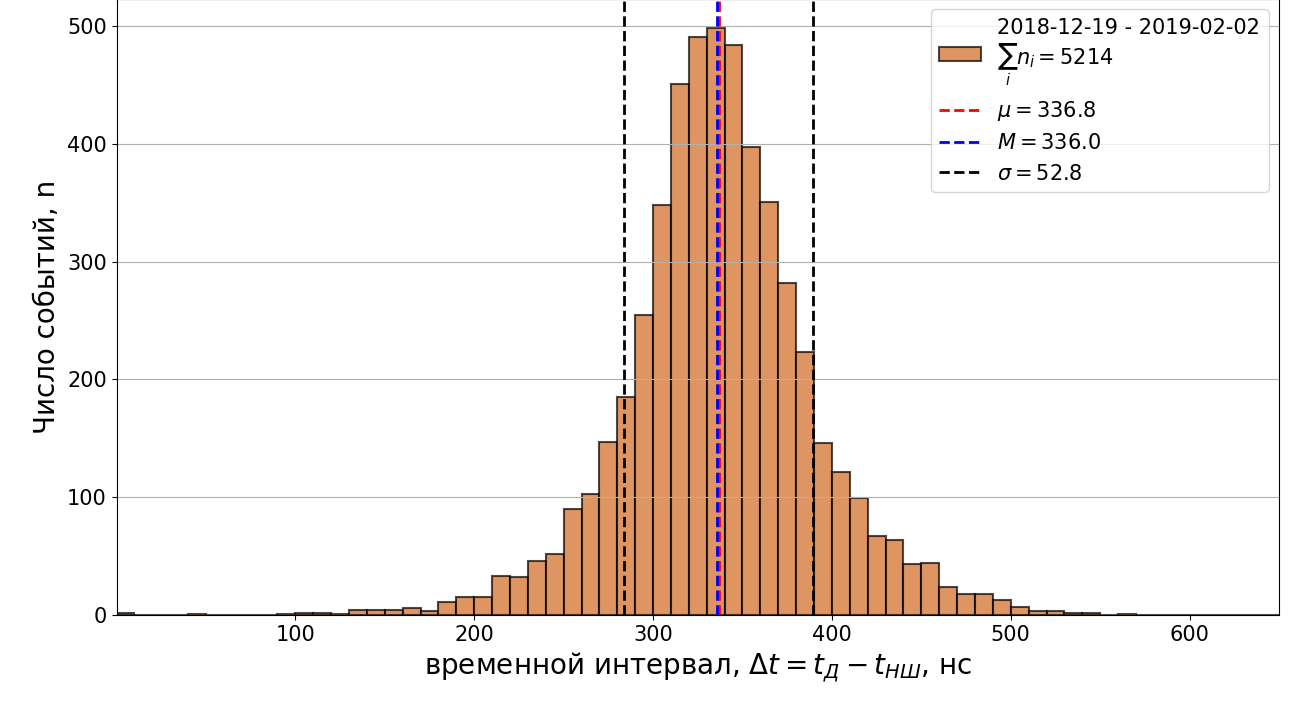
\includegraphics[width=0.9\textwidth]{images/events_by_delta_time.png}
    \caption{Распределение числа совместных событий по временному интервалу между событиями на установках ДЕКОР и НЕВОД-ШАЛ}
    \label{fig:your_image_label}
\end{figure}

Были определены совместные события с группами мюонов \(m > 5\). Распределение числа событий групп мюнов по номеру RUN и его длительности изображено на рисунке 6.

\begin{figure}[ht]
    \centering
    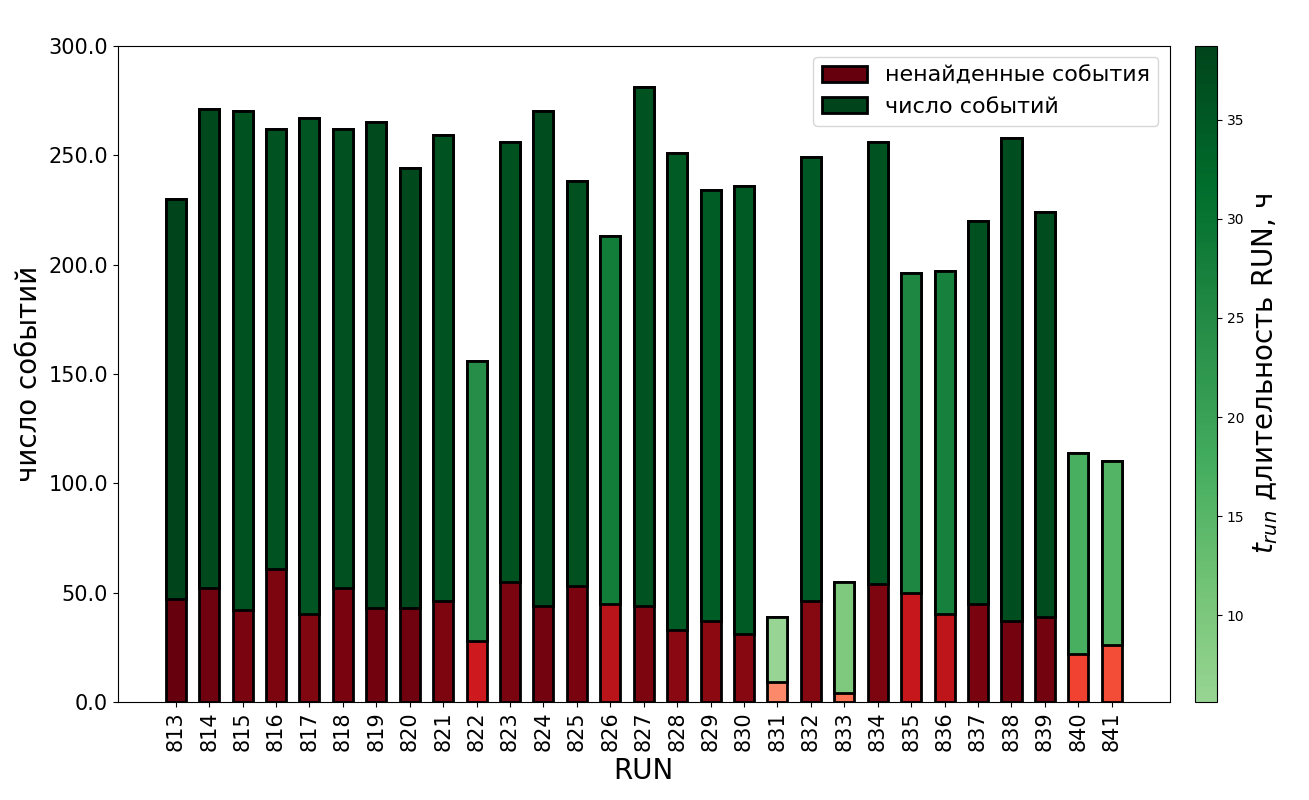
\includegraphics[width=0.9\textwidth]{images/muon_group_by_run.png}
    \caption{Распределение числа событий групп мюнов по номеру RUN}
    \label{fig:muon_group_by_run}
\end{figure}


\begin{figure}[h]
    \centering
    \subfloat[]{%
        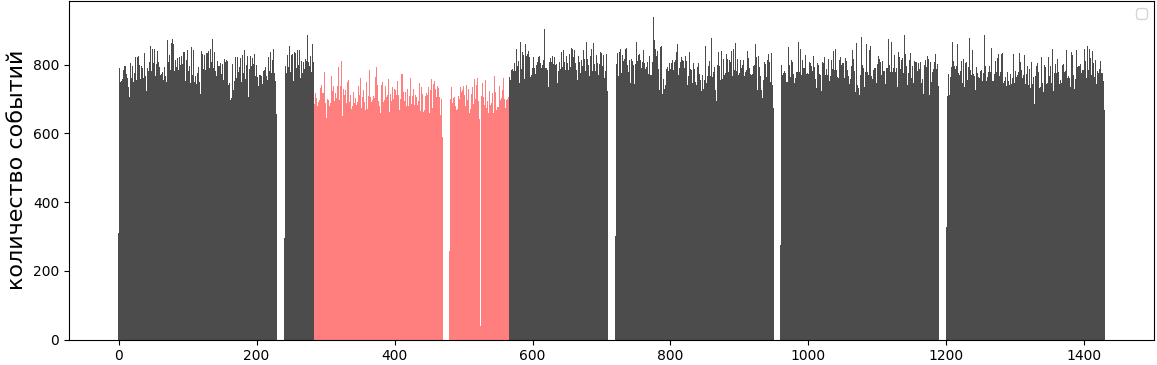
\includegraphics[width=0.9\textwidth, keepaspectratio]{images/19.12.18.png}%
        \label{fig:muon_group1}%
    }%

    \subfloat[]{%
        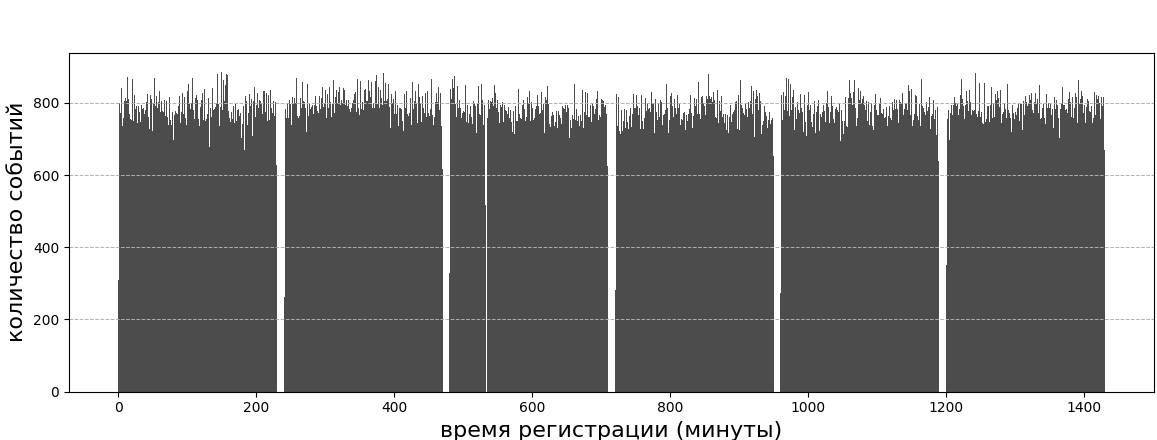
\includegraphics[width=0.9\textwidth, keepaspectratio]{images/20.12.18.png}%
        \label{fig:muon_group}%
    }%

    \caption{Темп счета событий установки НЕВОД-ШАЛ за 19.12.2018 (а) и 20.12.2018 (б)}
    \label{fig:muon_example}
\end{figure}
Можно отметить, что примерно для 20\% событий групп мюонов не было найдено совместных событий на установке НЕВОД-ШАЛ. Для определения причин данного явления был проведен первичный анализ не найденных событий. 

Установка НЕВОД-ШАЛ может работать как в режиме экспозиции, так и мониторинга. Интервалы работы установки в режиме экспозиции разбиваются на временные отрезки длительностью 10 минут, в ходе которых не происходит срабатываний детектирующих станций.
На рисунке 7 представлен темп счета регистрации событий на установке НЕВОД-ШАЛ за 19.12.2018 (а) и 20.12.2018 (б). Видно, что 20.12.2018 (б) установка имеет стабильный в течение всего дня темпы счета, когда за 19.12.2018 (а) имеется резкий спад, что может быть вызвано с временными техническими неисправностями некоторых детектирующий станций. 

Учитывая выше описанные особенности работы установки НЕВОД-ШАЛ, было построено распределение зенитного угла \(\theta\) направлений прихода событий для групп мюонов с отсутствующими совместными событиями на установке НЕВОД-ШАЛ за 19.12.2018 и 20.12.2018 числа (рисунок 8). 

 Из-за меньшей проникающей способности электронно-фотонной компоненты, часть отсутствующих совместных событий установки НЕВОД-ШАЛ можно списать на высокие зенитные углы. 
 \newpage
\begin{figure}[h]
    \centering
    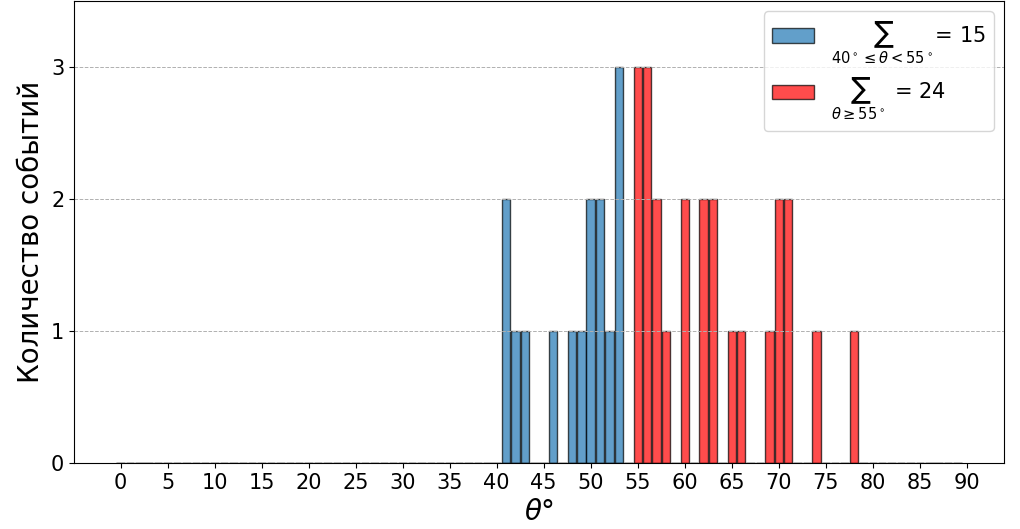
\includegraphics[width=0.85\textwidth]{images/not_events_by_theta.png}
    \caption{Распределение числа событий с группами мюонов без совместного события на установке НЕВОД-ШАЛ по зенитному углу \(\theta\)}
    \label{fig:not_events_by_theta}
\end{figure}
\begin{figure}[h]
    \centering
    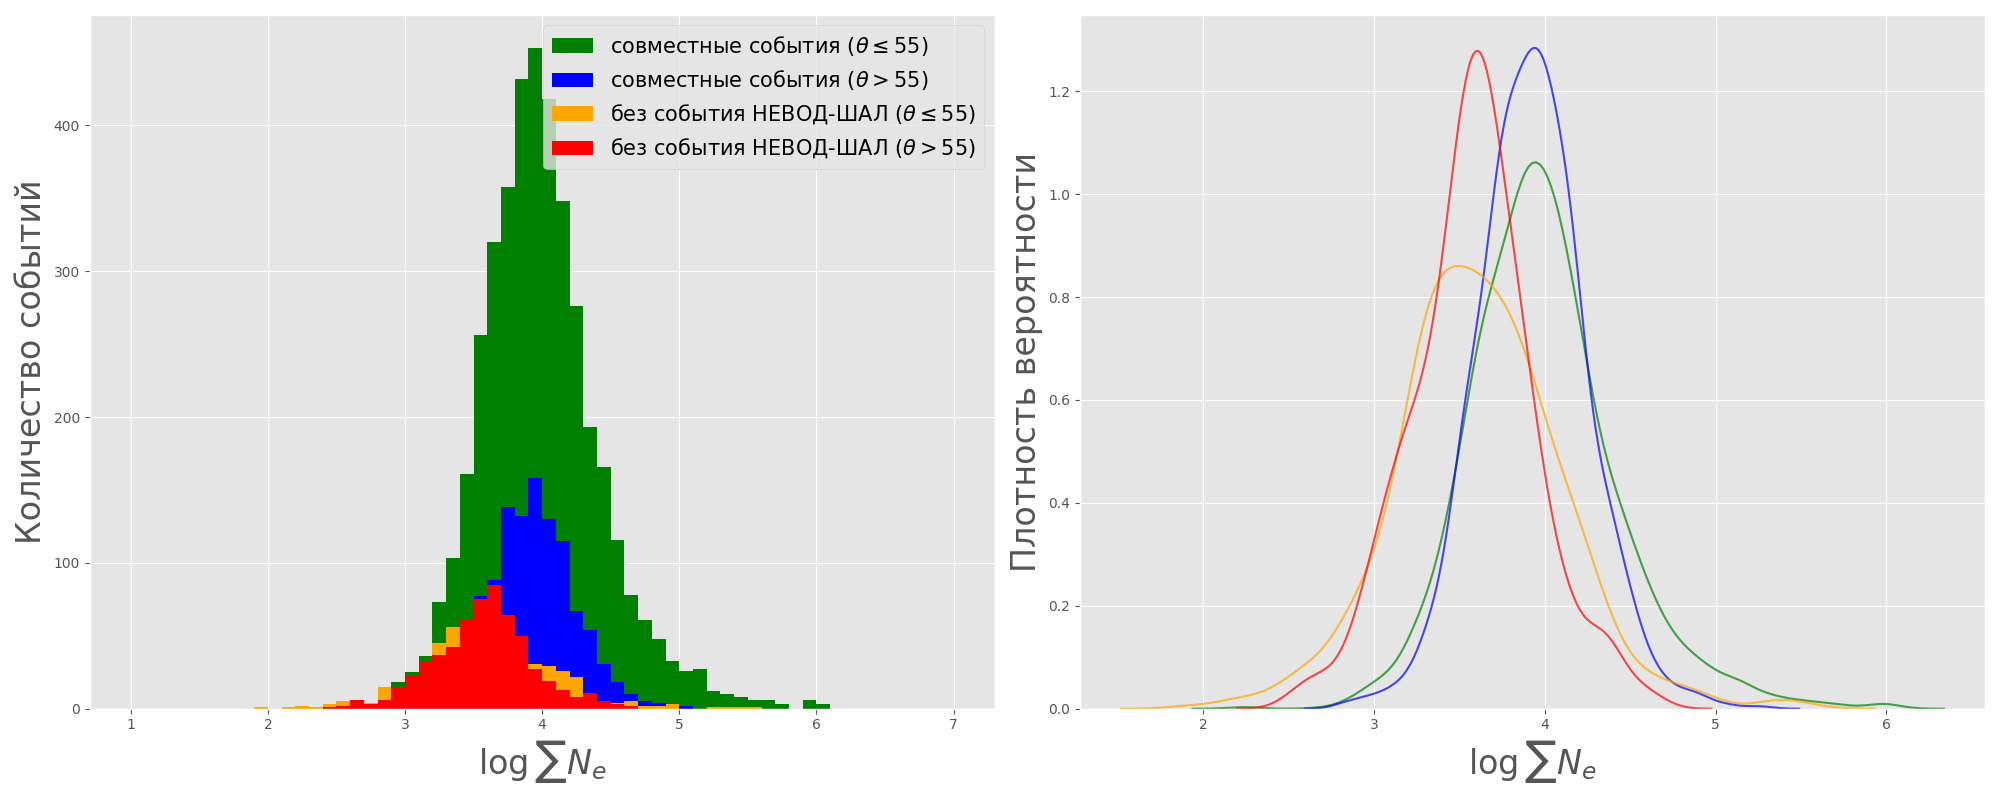
\includegraphics[width=1\textwidth]{images/logQ_theta55.png}
    \caption{Распределения числа событий (слева) и плотности вероятности событий (справа) по десятичному логарифма суммарного сигнала фотоумножителей событий с группами мюонов на ЧВД НЕВОД}
    \label{fig:logQ_theta55}
\end{figure}
\begin{figure}[h]
    \centering
    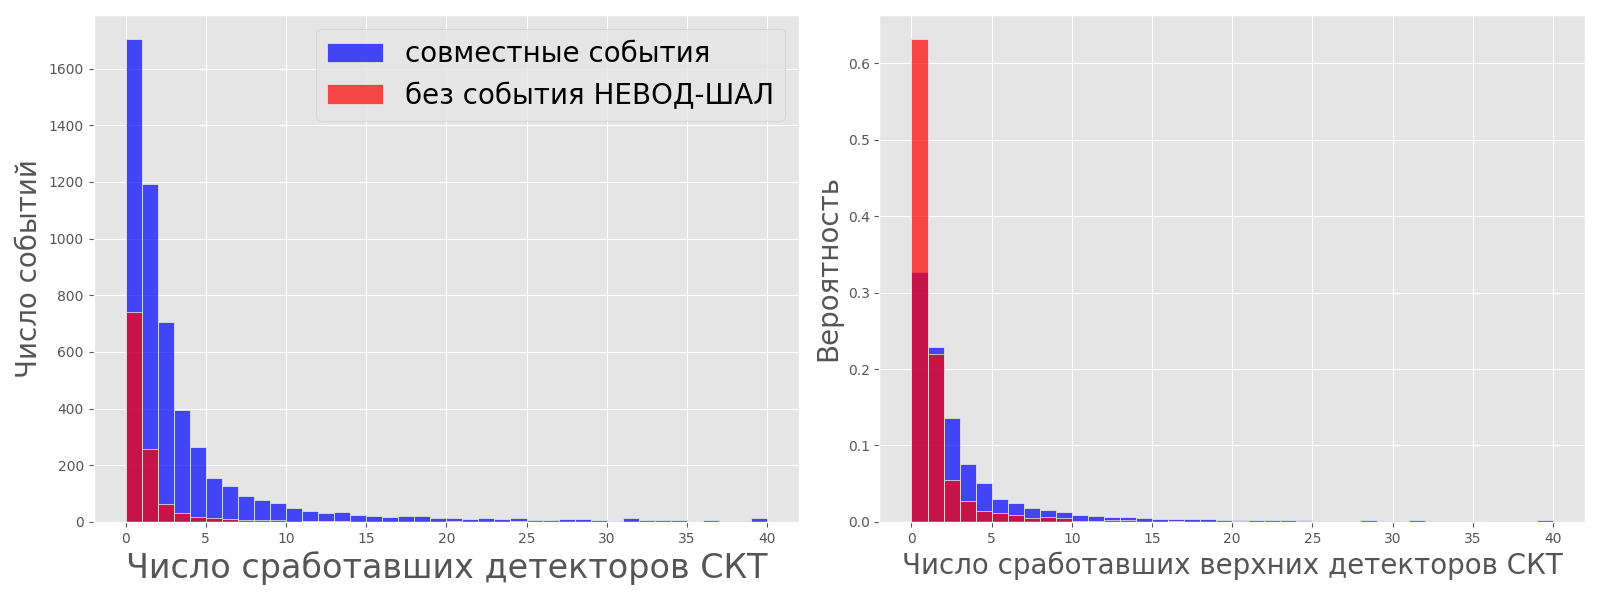
\includegraphics[width=1\textwidth]{images/SKT.png}
    \caption{Распределения числа событий (слева) и плотности вероятности событий (справа) по десятичному логарифма суммарного сигнала фотоумножителей событий с группами мюонов на ЧВД НЕВОД}
    \label{fig:SKT.png}
\end{figure}
\newpage
 
Были рассмотрены отклики на установке ЧВД НЕВОД и детекторах СКТ событий с группами мюонов. На рисунке 9 представлены распределения числа событий (слева) и плотности вероятности событий (справа) по десятичному логарифма суммарного сигнала фотоумножителей событий с группами мюонов на ЧВД НЕВОД.
На рисунке 10 представлены распределения числа событий (слева) и вероятности событий (справа) по числу сработавших верхних детекторов СКТ.
\endinput
